\chapter{Dynamic Schedules}
\label{chap:Dynamic}
The static schedule presented in Chapter~\ref{chap:Static} and applied commonly in the scheduled arrivals literature is fixed for the duration of service. It would intuitively be advantageous to allow the schedule to vary during service. For example, if the service times of the first few customers are longer than expected, then it would be beneficial to schedule the remaining customers to arrive later.

This chapter approaches the problem of choosing a schedule in a similar way to Chapter~\ref{chap:Static}. The aim is to find the arrival time of the first customer and the customer interarrival times that minimise the expected cost. The assumptions of iid service times and punctual customers are the same as Chapter~\ref{chap:Static}.

The dynamic schedule is chosen progressively during service. Immediately after a customer arrives and begins waiting for service, the scheduler chooses the arrival time of the next customer. Most real-world situations are obviously more restrictive than this. It is often not possible to schedule the customer arrivals one-by-one.

Real-world situations may sometimes allow a degree of flexibility in regards to rescheduling customers. The theory is that if the dynamic schedule presented here is significantly better than the static schedule, than (if possible) the rescheduling ability should be included in real-world models for scheduled arrivals. However, if the dynamic schedule performs similarly to the static schedule than it is likely reasonable to ignore the rescheduling in the model formulation.

\section{Markov Decision Process}
We consider the problem of scheduling $M$ customers. Denote the number of customers in the system on arrival of customer $i$ by $k_{i}$. In a similar way to the sequence $\{ N_{i} \}$ in Chapter~\ref{chap:Static}, the sequence $\{ k_{1}, \ldots, k_{M} \}$ is a discrete time Markov chain with a finite horizon. In contrast to Chapter~\ref{chap:Static}, we follow the general convention here and define $\{ k_{i} \}$ to be a right-continuous process with left limits.

We denote the states of the Markov chain as $(n, k)$. This state refers to $n$ customers remaining to be scheduled and $k$ customers currently in the system (i.e., either waiting or being served). The state variable $n$ is treated as the current `time' of the Markov chain. On arrival of the first customer, the system is in state $(M - 1, k_{1})$. On arrival of the second customer, the system is in state $(M - 2, k_{2})$. On arrival of the last customer, the system is in state $(0, k_{M})$.

For $n \geq 1$, at each state $(n, k)$ the scheduler needs to schedule the arrival of the next customer relative to the current time. We denote this time (i.e., action) by $a$. The scheduler cannot schedule the customer to arrive in the past so the set of possible actions is $A = [0, \infty)$. The time $a$ must be chosen such that $a \in A$.

This process is naturally modelled as a Markov decision process. The aim is to find a policy for the scheduler to choose the optimal value of $a$. Denote the optimal policy by $a^{*}$.

\section{Expected Cost of Schedule}
As in Chapter~\ref{chap:Static}, the expected cost of a schedule is a linear combination of the expected total customers' waiting time and the expected server availability time. Denote the expected cost of the state $(n, k)$ given that the next customer is scheduled to arrive in $a$ time units by $C_{n} (a, k)$. The optimal policy minimises the expected cost of the state $(n, k)$. Denote this minimum by $C_{n}^{*} (k)$ such that
\begin{equation}
	C_{n}^{*} (k) = C_{n} (a^{*}, k) = \min_{a \geq 0} C_{n} (a, k).
\end{equation}

Each transition in the Markov chain decrements the value of $n$ and transitions to a new value of $k$. Suppose the next customer is scheduled to arrive in $a$ time units. Consider the transition from state $(n, k)$ to state $(n - 1, j)$ over time interval $a$. Denote the probability of this transition by $p_{a} (k, j)$, and the expected cost during this transition by $R_{a} (k, j)$. Note that $j$ is the total number of customers in the system immediately after the next customer's arrival.

Bellman's Principle of Optimality \citep{Sniedovich} states that
\begin{quote}
	An optimal policy has the property that, whatever the initial state and initial decision are, the remaining decisions must constitute an optimal policy with regard to the state resulting from the first decision.
\end{quote}

This implies that the expected cost of the current state (under the optimal policy) is a function of the expected cost involved in transitioning to the next state, the expected cost of the next state (under the optimal policy) and the probability of transitioning to the next state over all possible next states.

For $n \geq 1$, the expected cost of state $(n, k)$ can be computed by the Bellman equation \citep{Bellman},
\begin{equation}
	C_{n}^{*} (k) \coloneqq \min_{a \geq 0} C_{n} (a, k) = \min_{a \geq 0} \left[ \sum_{j = 1}^{k + 1} p_{a} (k, j) \Big( R_{a} (k, j) + C_{n - 1}^{*} (j) \Big) \right].
	\label{Eqn_Bellman}
\end{equation}

Equation~\ref{Eqn_Bellman} is a recursive equation involving $C^{*}$. The optimal dynamic schedule is found by solving for each optimal interarrival time $a$ iteratively.

\section{Base Case}
Solving Equation~\ref{Eqn_Bellman} requires a solution for the base case where $n = 0$. The state $(0, k)$ is the state where there are no customers remaining to be scheduled and $k$ customers currently in the system. No futher scheduling decisions are required at this state.

Denote the expected waiting time of the customer that is currently in position $i$ as $w_{i}$. This expected waiting time is the summation of the expected service times of all the customers in positions $\{ 1, \ldots, i - 1 \}$. The expected total customers' waiting time for the $k$ remaining customers is the sum of their individual waiting times,
\begin{align}
	\begin{split}
		\mathbb{E} \Big[\text{total customer's waiting time at state $(0, k)$} \Big] & = \sum_{i = 1}^{k} w_{i} \\
		& = \sum_{i = 1}^{k} \mu (i - 1) \\
		& = \frac{\mu k (k - 1)}{2}.
	\end{split}
\end{align}

If there are no customers remaining to be scheduled, then the expected server availability time is the expected time until the customer currently in the last position in the queue finishes service. This time is the summation of the expected service times of the $k$ customers currently in the system,
\begin{equation}
	\mathbb{E} \Big[\text{server availability time at state $(0, k)$} \Big] = \sum_{i = 1}^{k} \mu = k \mu.
\end{equation}

The per unit time costs $c_{W}$ and $c_{S}$ are defined as before in Chapter~\ref{chap:Static}. The expected cost of the base case is thus given by
\begin{equation}
 	C_{0}^{*} (k) = c_{W} \frac{\mu k (k - 1)}{2} + c_{S} k \mu.
\end{equation}

In order to compare $C_{0}^{*} (k)$ with the cost of the static schedule, need to scale it by dividing by $(c_{S} + c_{W})$ and defining $\gamma = \frac{c_{S}}{c_{S} + c_{W}}$,
\begin{equation}
	C_{0}^{*} (k) \coloneqq (1 - \gamma) \frac{\mu k (k - 1)}{2} + \gamma k \mu.
\end{equation}

\section{Erlang Distribution}
The transition probability and expected transition cost for the dynamic schedule depend on the distribution function and conditional expectations of the Erlang distribution, which are shown here.

Denote the service time of the customer that is currently in position $i$ in the queue as $S_{i}$. For $n$ customers, the service times $S_{1}, \ldots, S_{n}$ are iid exponential random variables with mean $\mu$.

For $r \geq 1$, the waiting time of the customer in position $(r + 1)$ is given by
\begin{equation}
	X = \sum_{i = 1}^{r} S_{i} \sim \text{Erlang}(r, \mu),
\end{equation}

which has density
\begin{equation}
	f (x; r) \coloneqq \frac{1}{\mu (r - 1)!} \left( \frac{x}{\mu} \right)^{r - 1} \mathrm{e}^{\frac{-x}{\mu}},
\end{equation}

and distribution function
\begin{equation}
	F (x; r) \coloneqq \mathbb{P} (X \leq x) = \begin{cases} 0 & \text{for $x = 0$} \\ 1 - \sum_{i = 0}^{r - 1} \frac{1}{i!} \left( \frac{x}{\mu} \right)^{i} \mathrm{e}^{\frac{-x}{\mu}} & \text{for $x > 0$}. \end{cases}
\end{equation}

For $x \geq 0$, $F (x; r)$ is continuous as
\begin{equation}
	\lim_{x \to 0^{+}} F (x; r) = 0 = F (0; r).
\end{equation}

Computing the expected transition cost requires the conditional expectation of $X$ given $X \leq a$. We are unable to find reference to this conditional expectation in the literature so derive it here (for $a > 0$),
\begin{align}
	\begin{split}
		\mathbb{E} [X | X \leq a]
		& = \int x \ \mathbb{P} (X \in d x | X \leq a) \\
		& = \frac{1}{\mathbb{P} (X \leq a)} \int x \ \mathbb{P} (X \in d x, X \leq a) \\
		& = \frac{1}{F (a; r)} \int_{0}^{a} x f(x; r) d x \\
		& = \frac{\mu r}{F (a; r)} \int_{0}^{a} \frac{1}{\mu r!} \left( \frac{x}{\mu} \right)^{r} \mathrm{e}^{\frac{-x}{\mu}} d x \\
		& = \frac{\mu r F (a; r + 1)}{F (a; r)}.
	\end{split}
\end{align}

Moreover, $\mathbb{E} [X | X \leq 0] = 0$ by definition. Therefore, the conditional expectation of $X$ given $X \leq a$ is defined as
\begin{equation}
	G (a; r) \coloneqq \mathbb{E} [X | X \leq a] = \begin{cases} 0 & \text{for $a = 0$} \\ \frac{\mu r F (a; r + 1)}{F (a; r)} & \text{for $a > 0$}. \end{cases}
\end{equation}

This expression makes intutive sense. For $a > 0$ and $r \geq 1$, $\frac{F (a; r + 1)}{F (a; r)} < 1$. In addition, the mean of the Erlang distribution is $\mathbb{E} [X] = \mu r$. Thus, for $a > 0$ and $r \geq 1$, $\mathbb{E} [X | X \leq a] < \mathbb{E} [X]$ as expected.

Moreover, 
\begin{equation}
	\lim_{a \to \infty} \frac{F (a; r + 1)}{F (a; r)} = \frac{\displaystyle \lim_{a \to \infty} F (a; r + 1)}{\displaystyle \lim_{a \to \infty} F (a; r)} = \frac{1}{1} = 1.
\end{equation}

Thus, $\displaystyle \lim_{a \to \infty} \mathbb{E} [X | X \leq a] = \mathbb{E} [X]$ as expected.

Finally, suppose there is an exponential random variable $Y$ with mean $\mu$ that is independent of $X$. The expected transition cost also requires the conditional expectation of $X$ given $X \leq a$ and $X + Y > a$. We were again unable to find reference to this conditional expectation in the literature so derive it here (for $a > 0$),
\begin{align}
	\begin{split}
		& \ \mathbb{E} [X | X \leq a, X + Y > a] \\
		= & \ \int x \ \mathbb{P} (X \in d x | X \leq a, X + Y > a) \\
		= & \ \frac{1}{\mathbb{P} (X \leq a, X + Y > a)} \int x \ \mathbb{P} (X \in d x, X \leq a, X + Y > a) \\
		= & \ \frac{1}{\mathbb{P} (X \leq a, X + Y > a)} \iint_{D} x \ \mathbb{P} (X \in d x, X \leq a, X + y > a) f (y; 1) d y.
	\end{split}
\end{align}

The double integral needs to be evaluated over
\begin{equation}
	D = \Big\{ (x, y) : x \geq 0, y \geq 0, x \leq a, x + y > a \Big\}.
\end{equation}

$D$ can be expressed as the union of two disjoint sets in the following way,
\begin{equation}
	D = \Big\{ (x, y) : x \in (a - y, a], y \in [0, a] \Big\} \bigcup \Big\{ (x, y) : x \in [0, a], y \in (a, \infty) \Big\}.
\end{equation}

In addition, we show in the appendix that
\begin{equation}
	\mathbb{P} (X \leq a, X + Y > a) = \frac{1}{r!} \left( \frac{a}{\mu} \right)^{r} \mathrm{e}^{\frac{-a}{\mu}}.
\end{equation}

Thus, the conditional expectation can be further derived below,
\begin{align}
	\begin{split}
		& \ \mathbb{E} [X | X \leq a, X + Y > a] \\
		= & \ \frac{1}{\ \frac{1}{r!} \left( \frac{a}{\mu} \right)^{r} \mathrm{e}^{\frac{-a}{\mu}}} \left[ \int_{0}^{a} \int_{a - y}^{a} + \int_{a}^{\infty} \int_{0}^{a} \right] x f (x; r) f (y; 1) d x d y \\
		= & \ \frac{\frac{a}{r + 1} \frac{1}{(r - 1)!} \left( \frac{a}{\mu} \right)^{r} \mathrm{e}^{\frac{-a}{\mu}}}{\frac{1}{r!} \left( \frac{a}{\mu} \right)^{r} \mathrm{e}^{\frac{-a}{\mu}}} \\
		= & \ \frac{a r}{r + 1}.
	\end{split}
\end{align}

Moreover, $\mathbb{E} [X | X \leq 0, X + Y > 0] = 0$ by definition. Therefore, the conditional expectation of $X$ given $X \leq a$ and $X + Y > a$ is defined as
\begin{equation}
	H (a; r) \coloneqq \mathbb{E} [X | X \leq a, X + Y > a] = \frac{a r}{r + 1}.
\end{equation}

Perhaps surprisingly, the conditional expectation $H (a; r)$ does not depend on the parameter $\mu$.

\section{Transition Probability}
The transition probability $p_{a} (k, j)$ is the probability that the number of customers in the system changes from $k$ customers initially to $j$ customers on the arrival of the next customer after $a$ time units. In other words, it is the probability that there are $k - (j - 1)$ departures from the queue over a time interval of length $a$.

The transition probability is most easily derived on a case by case basis. The full derivation is included in the appendix and only the final equation is presented here,
\begin{equation}
	p_{a} (k, j) \coloneqq \begin{cases}
		\mathbbm{1} (j = 1) & \text{for $k = 0$} \\
		F (a; k) & \text{for $k \geq 1, j = 1$} \\
		F (a; k - j + 1) - F (a; k - j + 2) & \text{for $k \geq 2, 2 \leq j \leq k$} \\
		1 - F (a; 1) & \text{for $k \geq 1, j = (k + 1)$} \\
		0 & \text{otherwise}.
	\end{cases}
\end{equation}

Given a current state $(n, k)$ and a time interval $a$, the total probability over all possible next states $\big\{ (n - 1, j) : 1 \leq j \leq k + 1 \big\}$ is
\begin{equation}
	\sum_{j = 1}^{k + 1} p_{a} (k, j) = 1.
\end{equation}

\section{Expected Transition Cost}
The expected transition cost is the expected cost of transitioning from state $(n, k)$ to state $(n - 1, j)$ if the next customer is scheduled to arrive in $a$ time units.

In a similar way to the transition probability, the expected transition cost is derived on a case by case basis. To compare the dynamic schedule with the static schedule, the cost is scaled by dividing by $(c_{S} + c_{W})$ and defining $\gamma = \frac{c_{S}}{c_{S} + c_{W}}$. The full derivation is included in the appendix and the final equation is presented here,
\begin{equation}
	R_{a} (k, j) \coloneqq \begin{cases}
		\gamma a & \text{for $k \in \{ 0, 1 \}$} \\
		(1 - \gamma) \frac{G (a; k) (k - 1)}{2} + \gamma a & \text{for $k \geq 2, j = 1$} \\
		(1 - \gamma) \frac{a (k + j - 3)}{2} + \gamma a & \text{for $k \geq 2, 2 \leq j \leq k + 1$}.
	\end{cases}
\end{equation}

\section{Example Models}
\subsection{Model for 2 Customers}
Assume there are two customers that need to be scheduled for service. The initial state is $(2, 0)$ (i.e., two customers to schedule and no customers currently in the system). The possible states during service are all the states in the set
\begin{equation}
	\Big\{ (n, k) \in \{ 0, 1, 2 \}^{2} : n + k \leq 2 \Big\}.
\end{equation}.

From Equation~\ref{Eqn_Bellman}, for $n \geq 1$, the expected cost of state $(n, 0)$ (i.e., no customers currently in the system) as a function of the time interval $a$ until the next customer arrival is given by
\begin{equation}
	C_{n} (a, 0) = C_{n - 1}^{*} (1) + \gamma a.
\end{equation}

As $\gamma \in (0, 1)$, the optimal policy $a^{*}$ where $C_{n} (a, 0)$ attains a minimum is
\begin{equation}
	a^{*} = \argmin_{a \geq 0} C_{n} (a, 0) = 0.
	\label{eqn:Dynamic_No_Waiting}
\end{equation}

Thus, if there are no customers currently waiting, then the next customer should be scheduled to arrive immediately. This agrees with the result of the static schedule that the first customer should be schedule to arrive immediately at the state of service.

As the transition occurs immediately, the expected cost of state $(n, 0)$ equals the expected cost of state $(n - 1, 1)$ for $n \geq 1$,
\begin{equation}
	C_{n}^{*} (0) = C_{n - 1}^{*} (1).
\end{equation}

From Equation~\ref{Eqn_Bellman}, for $n \geq 1$, the expected cost of state $(n, 1)$ (i.e., one customer currently in the system) as a function of the time interval $a$ until the next customer arrives is given by
\begin{equation}
	C_{n} (a, 1) = C_{n - 1}^{*} (1) + \mathrm{e}^{\frac{-a}{\mu}} \Big[ C_{n - 1}^{*} (2) - C_{n - 1}^{*} (1) \Big] + \gamma a.
\end{equation}

The optimal policy $a^{*}$ where $C_{n} (a, 1)$ attains a minimum is
\begin{equation}
	a^{*} = \argmin_{a \geq 0} C_{n} (a, 0) = \mu \ln \left[ \frac{C_{n - 1}^{*} (2) - C_{n - 1}^{*} (1)}{\gamma \mu} \right].
	\label{eqn:Dynamic_One_Waiting}
\end{equation}

Returning to the case of scheduling two customers using this dynamic schedule. By Equation~\ref{eqn:Dynamic_No_Waiting}, the first customer should be scheduled to arrive immediately. On the first customer's arrival, the system is at state $(1, 1)$. By Equation~\ref{eqn:Dynamic_One_Waiting}, the second customer should be scheduled to arrive $a^{*}$ after the arrival of the first customer where
\begin{equation}
	a^{*} = \mu \left[ \frac{C_{0}^{*} (2) - C_{0}^{*} (1)}{\gamma \mu} \right] = - \mu \ln \gamma.
\end{equation}

This dynamic schedule is exactly the same as the static schedule for two customers. As the first customer is scheduled to arrive at the start of service, all arrival times are decided at the start of service. Therefore, the optimal policy is the same for both schedules.

Unfortunately, for $k \geq 2$, no algebraic solution exists for the optimal policy for state $(n, k)$. Thus, we cannot analytically derive the dynamic schedule for more than two customers. Those cases need to be solved numerically.

To further illustrate this point, we consider the cost of the state $(1, 2)$ (i.e., one customer remaining to schedule and two customers currently in the system). From Equation~\ref{Eqn_Bellman}, the expected cost of this state as a function of the time until the last customer's arrival ($a$) is given by
\begin{equation}
	C_{1} (a, 2) = \gamma a + \mu + \mathrm{e}^{\frac{-a}{\mu}} (a + 2 \mu).
\end{equation}

The optimal policy $a^{*}$ where $C_{1} (a, 2)$ attains a minimum is given by the $a^{*}$ that solves the equation
\begin{equation}
	- \left( 1 + \frac{a^{*}}{\mu} \right) \mathrm{e}^{- \left( 1 + \frac{a^{*}}{\mu} \right)} = - \gamma \mathrm{e}^{-1}.
\end{equation}

The optimal policy can be defined in terms of the Lambert $W$ function as
\begin{equation}
	a^{*} = - \mu \left[ 1 + W \left( - \gamma \mathrm{e}^{-1} \right) \right].
\end{equation}

The Lambert $W$ function is the inverse function of
\begin{equation}
	f (W) = W \mathrm{e}^{W}.
\end{equation}

Unfortunately, $W$ is not an elementary function \citep{Chow}. The optimal arrival time of the last customer needs to be computed numerically for a given value of $\gamma$.

\subsection{Model for 15 Customers}
We consider here the case of $n = 15$. Without loss of generality, can let $\mu = 1$. For $\mu \neq 1$, the optimal policies $a^{*}$ found are the optimal interarrival times $\mu a^{*}$. For simplicity, assume that the per unit time costs $c_{W}$ and $c_{S}$ are both equal such that $\gamma = 0.5$.

In a similar way to Chapter~\ref{chap:Static}, we developed an algorithm in Python to efficiently find a numeric approximation to the optimal dynamic schedule. The algorithm is included in the appendix. We again use the `L-BFGS-B' method of $\texttt{scipy.optimize.minimize}$ in Python. Finding the optimal dynamic schedule for 15 customers involves solving several contrained optimisation problems. We solve for the optimal policy $a^{*}$ at each possible state in the set
\begin{equation}
	\Big\{ (n, k) \in \{ 0, \ldots, 15 \}^{2} : n + k \leq 15 \Big\}.
\end{equation}

Our algorithm finds the optimal policy at each of the states in the order given by
\begin{equation}
	(0, 0), (0, 1), \ldots, (0, 15), (1, 0), \ldots, (1, 14), (2, 1), \ldots, (14, 1), (15, 0).
\end{equation}

By choosing this order and storing the results of previous computations, our algorithm is able to easily find the dynamic schedule for $15$ customers. This algorithm is significantly more efficient than our algorithm for finding the optimal static schedule. Moreover, due to the nature of the dynamic schedule, the optimal schedule for scheduling $n = 15$ customers includes the optimal schedule for scheduling $n \leq 15$ customers.

We computed the expected cost of each state $(n, k)$ using our algorithm and the results are plotted in Figure~\ref{fig:Dynamic_Cost_15}.
\begin{figure}[htb]
	\centering
	\includegraphics[width = 0.85\textwidth]{Dynamic_Line_Cost_n.eps}
	\caption{Expected cost of possible states with $15$ total customers. Figure generated assuming $\gamma = \frac{c_{S}}{c_{S} + c_{W}} = 0.5$ and $\mu = 1$. Each line is plotted for a fixed value of the number of customers still to be scheduled ($n$). The darkest line is for $n = 0$. As $n$ increases, the lines become lighter.}
	\label{fig:Dynamic_Cost_15}
\end{figure}

The cost of the initial state $(15, 0)$ is $13.55$, thus the expected cost of serving $15$ customers with a dynamic schedule is $13.55$. The worst state in Figure~\ref{fig:Dynamic_Cost_15} is the state $(0, 15)$, which is all $15$ customers in the system. This can occur if all $15$ customers are scheduled to arrive immediately at the start of service (to ensure minimal server availability time) or if the first customer has an extremely long service time.

The lines plotted on Figure~\ref{fig:Dynamic_Cost_15} are the expected costs with fixed $n$ and varying $k$. As the number of customers in the system ($k$) increases, the expected cost increases exponentially. By contrast, as the number of customers to be scheduled ($n$) increases with $k$ fixed, the expected cost of the state increases approximately linearly at a significantly smaller rate.

It's difficult to observe, but for $n \geq 1$, Figure~\ref{fig:Dynamic_Cost_15} shows that $C_{n}^{*} (0) = C_{n - 1}^{*} (1)$. This confirms the previous result that if there are no customers currently in the system (e.g., initially), then it is always optimal to schedule the next arrival immediately. The expected cost does not change as the next arrival occurs immediately.

Figure~\ref{fig:Dynamic_Time_15} plots the corresponding interarrival times $a^{*}$ for the states plotted in Figure~\ref{fig:Dynamic_Cost_15}. This figure does not include optimal times for the states with $n = 0$ as there is no next customer to schedule in those states.
\begin{figure}[htb]
	\centering
	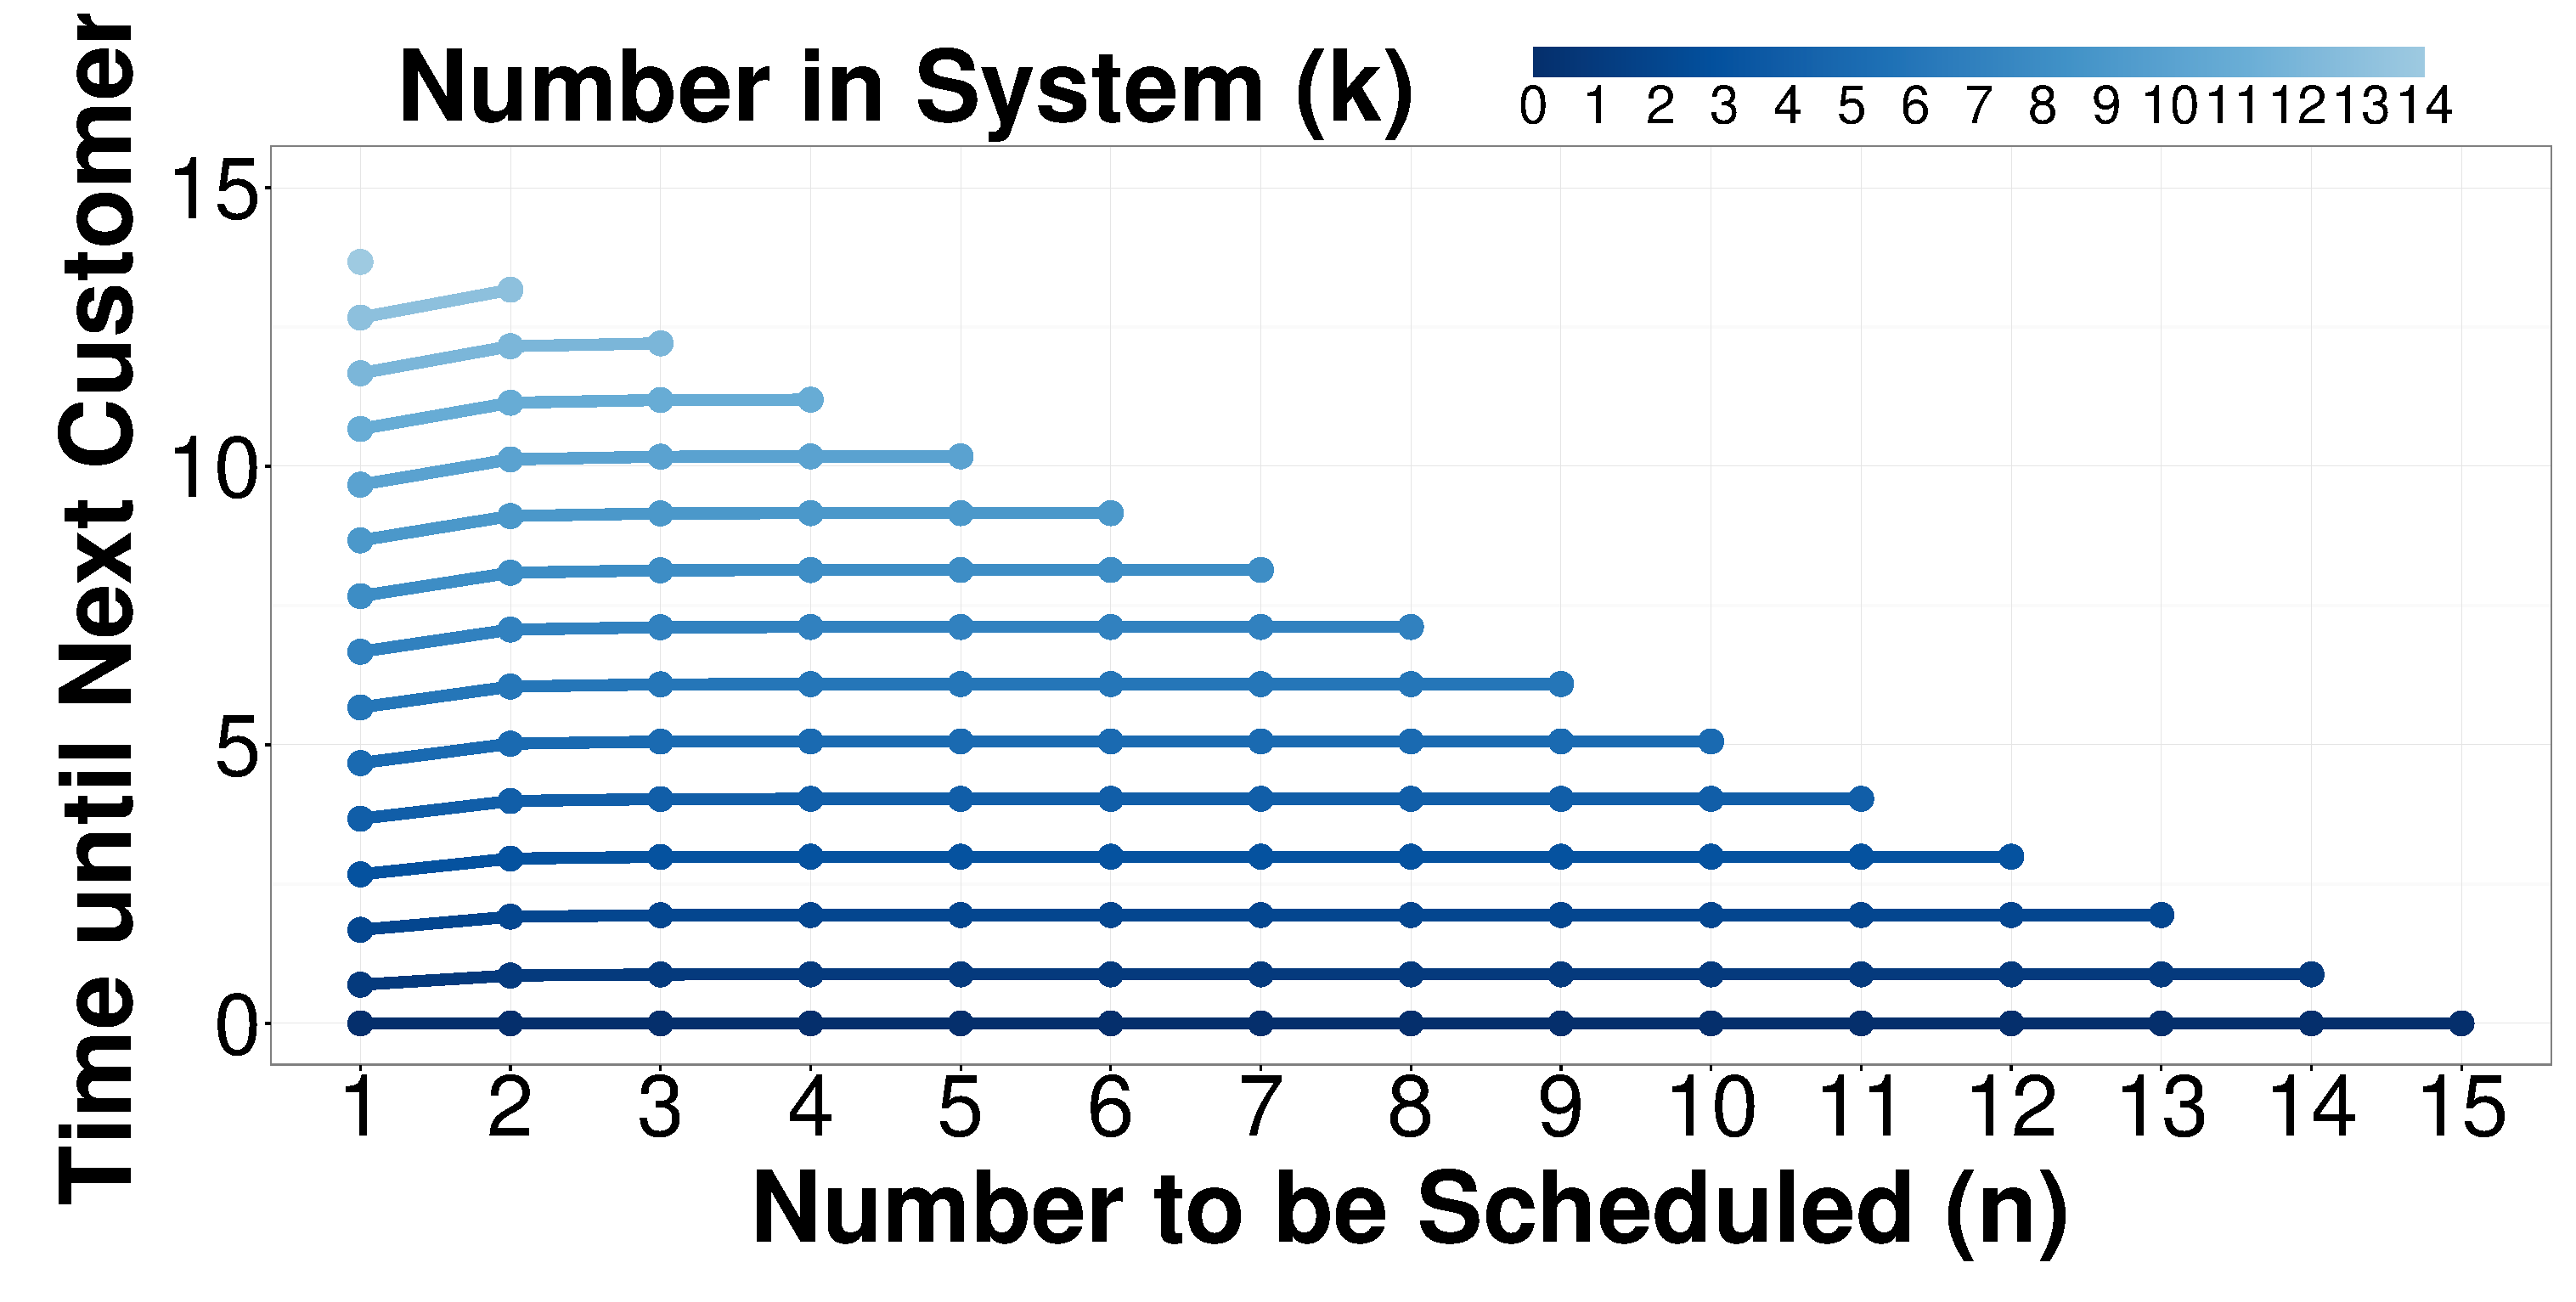
\includegraphics[width = 0.85\textwidth]{Dynamic_Line_Interarrival_k.eps}
	\caption{Optimal interarrival time for each possible state with $15$ total customers. Figure generated assuming $\gamma = \frac{c_{S}}{c_{S} + c_{W}} = 0.5$ and $\mu = 1$. Each line is plotted for a fixed value of the number of customers in the system ($k$). The darkest line is for $k = 0$. As $k$ increases, the lines become lighter.}
	\label{fig:Dynamic_Time_15}
\end{figure}

Understanding Figure~\ref{fig:Dynamic_Time_15} is helped by looking at some examples. The optimal interarrival time for the initial state $(15, 0)$ is $0$. The first customer should be scheduled to arrive immediately. The optimal interarrival time for the state $(3, 10)$ is $10.17$. If (on arrival of a customer), there are $10$ customers in the system and $3$ customers remaining to be scheduled, then the next customer should be scheduled to arrive in $10.17$ time units. This is slightly greater than the expected service time of the $10$ customers currently in the system to account for the customer waiting cost.

The first pattern to notice is that if there are no customers currently waiting (i.e., $k = 0$), then (as discussed earlier) the optimal policy is to schedule the next arrival immediately. This makes intutive sense as scheduling the next arrival immediately minimises the expected server availability time without effecting the expected total customers' waiting times.

As $k$ increases for fixed $n$, the optimal interarrival times $a^{*}$ appear to increase at a slightly decreasing rate. The optimal $a^{*}$ increases by approximately $\mu$ for each additional $k$. In contrast, for $n \geq 2$ and fixed $k$, $a^{*}$ appears to be constant at a value close to $\mu k$ (i.e., the expected time for the system to be empty). The optimal $a^{*}$ appears to be independent of the the number of customers still to be scheduled provided that there are at least two customers still to be scheduled.

































